\noindent
Wanneer de Autopilot een bol in beeld gekregen heeft, zal hij starten met zijn positie relatief tegenover zijn doel te bepalen. De werkwijze wordt in onderstaande beschrijving verduidelijkt.
\\
Ten eerst wordt de diepte bepaald. Dit kan met behulp van de formule van stereo vision \cite{website:techbriefs} berekend worden.
Zie Figuur \ref{fig:DiepteberekeningDroneEnDoel} voor een grafische weergave van de berekening. \(Z\) stelt de diepte [m] voor, \(c\) de afstand [m] tussen de camera's, \(f\) de focale afstand [pixel] en $x_1$ en $x_2$ stellen de afstand [pixel] tussen het middelpunt van het beeld en het middelpunt van de bol op het beeld voor. Het is eenvoudig in te zien dat de diepte berekend kan worden door formule \ref{eq: diepte}.
\begin{equation} \label{eq: diepte}
Z = \frac{c \cdot f}{x_1 - x_2}
\end{equation}
\begin{figure}[h]
	\centering
	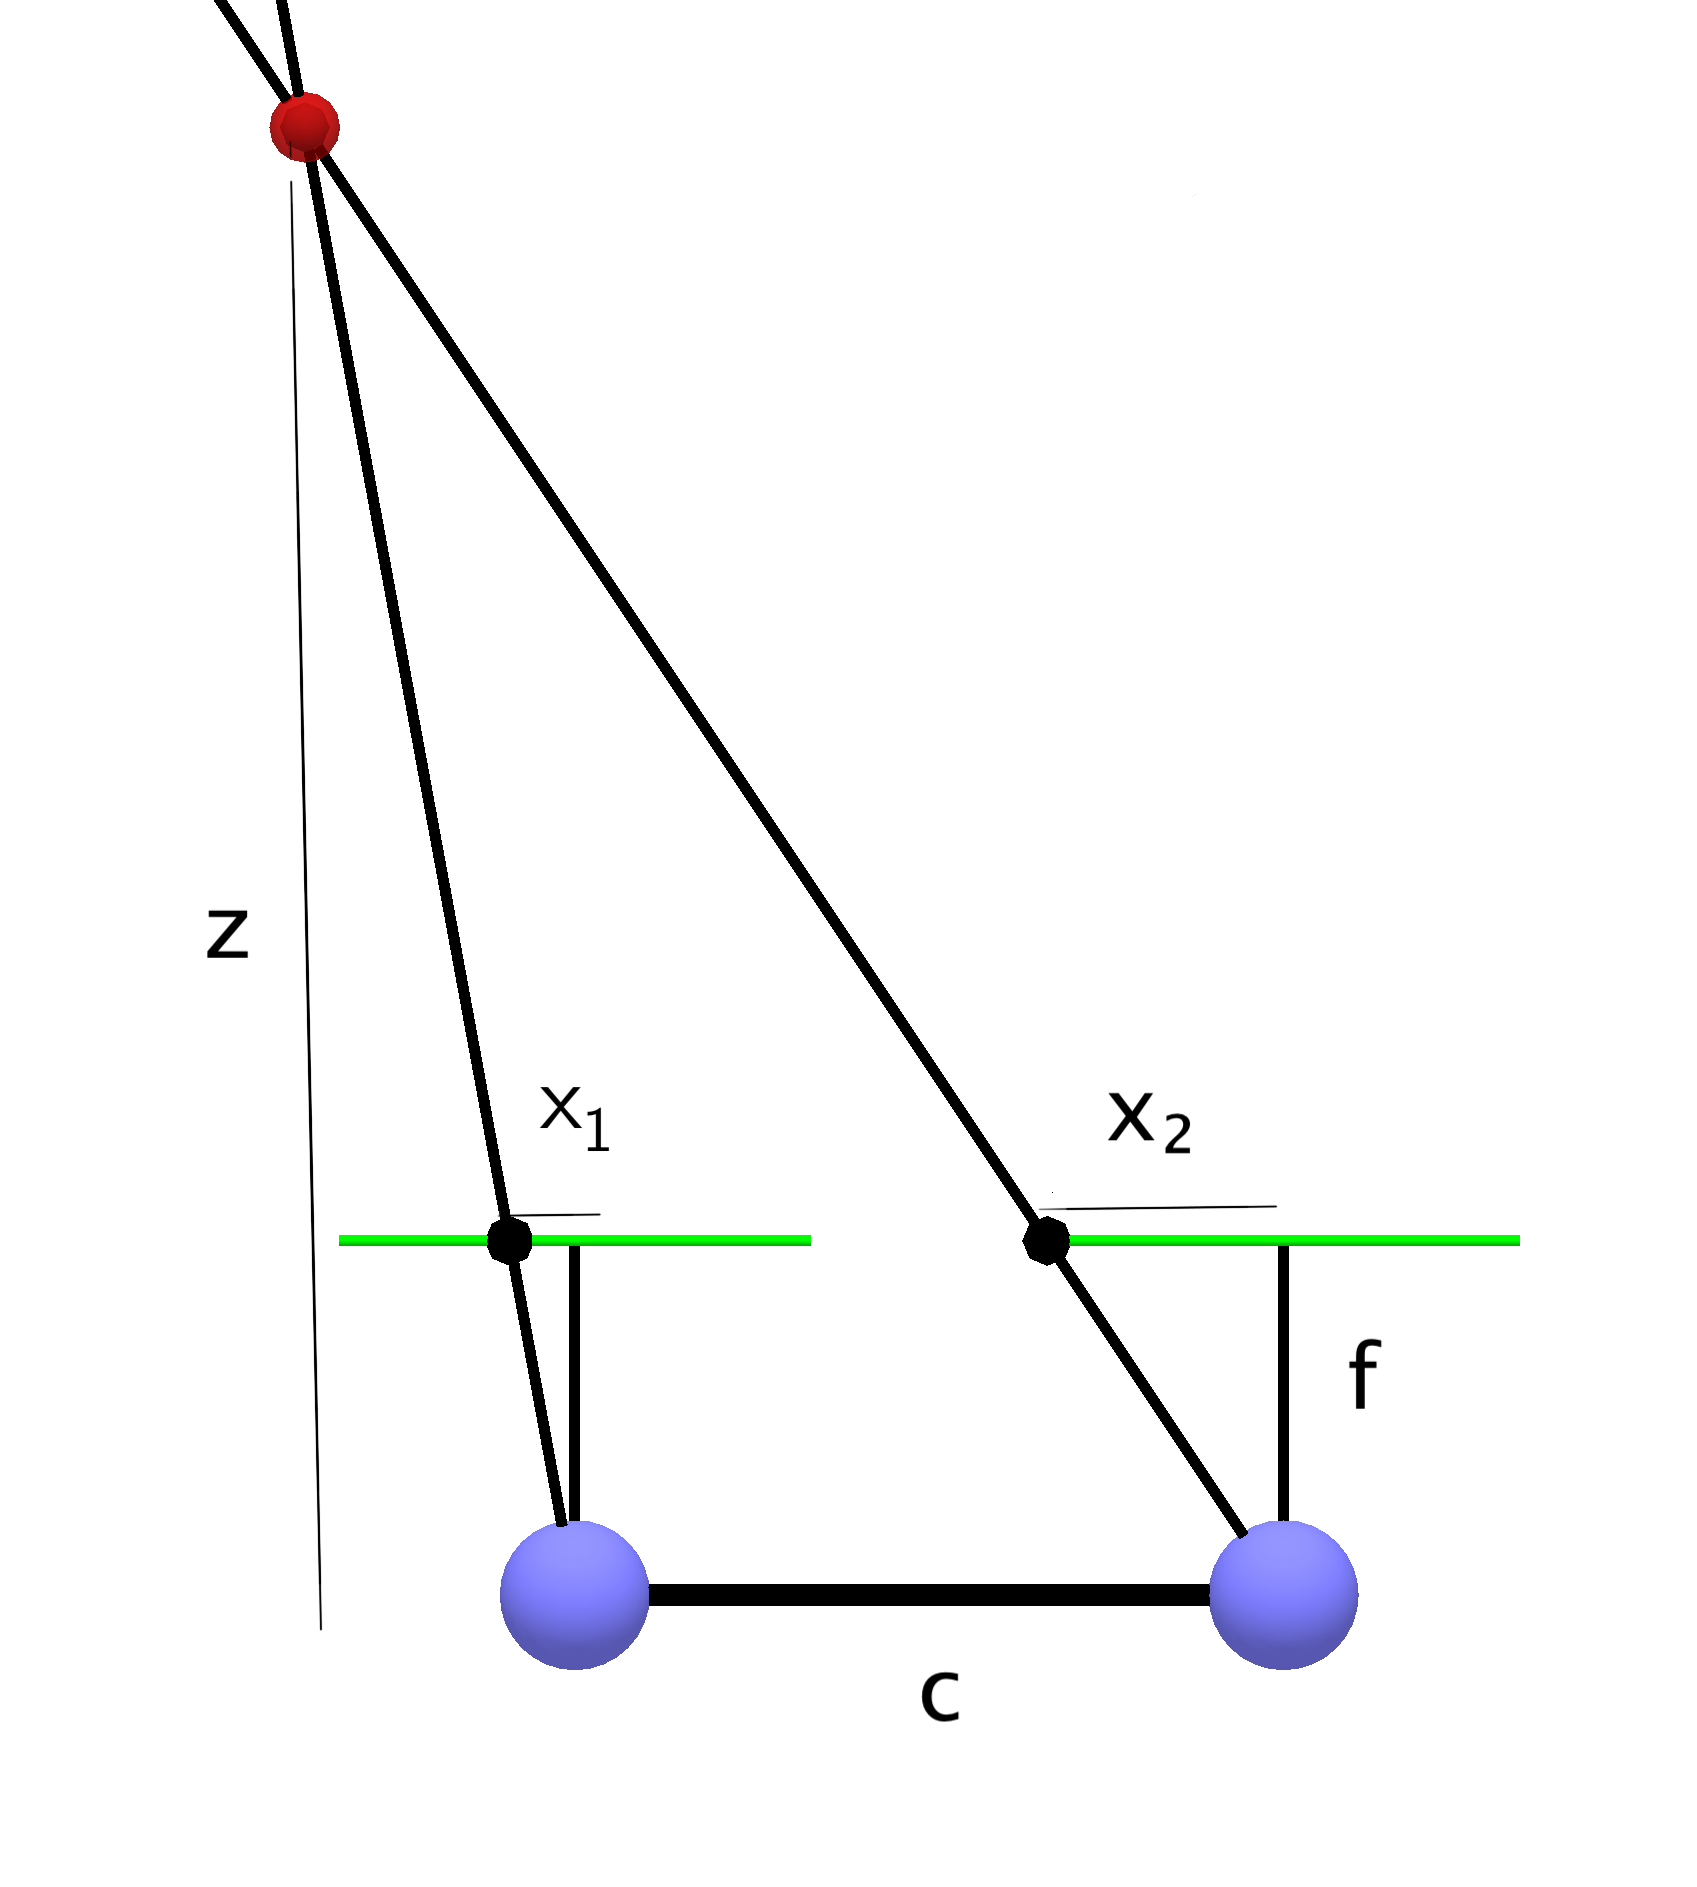
\includegraphics[width=0.3\textwidth]{DiepteberekeningDroneEnDoel.png}
	\caption{Diepteberekening tussen drone en doel. In formulevorm: \(Z = \frac{c \cdot f}{x_1 - x_2}\).}
	\label{fig:DiepteberekeningDroneEnDoel}
\end{figure}
\\
Vervolgens wordt de fout op de horizontale hoek, $\alpha$ bepaald. Hiermee wordt de afwijking tussen de horizontale positie van de bol en het midden van de drone bedoeld. Deze formule wordt afgeleid via de goniometrische regels. Zie Figuur \ref{fig:RelatieveHorizontaleHoek} voor grafische ondersteuning. De hoek $\delta$ stelt hier de helft van de horizontale hoek voor die het beeld overspant en b stelt de helft van de breedte van het beeld voor. Onder Figuur \ref{fig:RelatieveHorizontaleHoek} kan eveneens de uitwerking van de formule gevonden worden.
\\
Ten slotte wordt ook de fout op de verticale hoek, $\beta$ bepaald. Dit is de afwijking van de hoogte van de bol ten opzichte van de hoogte van de drone. Wederom afgeleid via de goniometrie en weergegeven in Figuur \ref{fig:RelatieveVerticaleHoek}, met $y_2$ de verticale afstand [pixel] tussen de het middelpunt van het beeld en het middelpunt van de bol.
\begin{figure}[h]
	\centering
	\begin{minipage}{.45\textwidth}
		\centering
		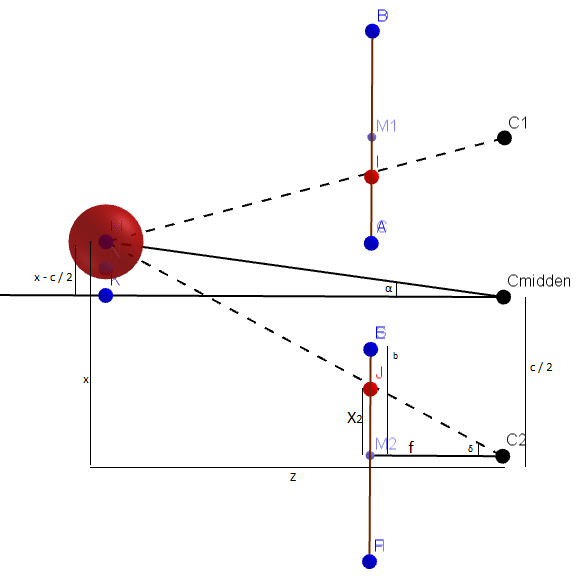
\includegraphics[width=1\textwidth]{RelatieveHorizontaleHoek.png}
		\caption{Relatieve horizontale hoek.}
		\label{fig:RelatieveHorizontaleHoek}
	\end{minipage}
	\begin{minipage}{.45\textwidth}
		\centering
		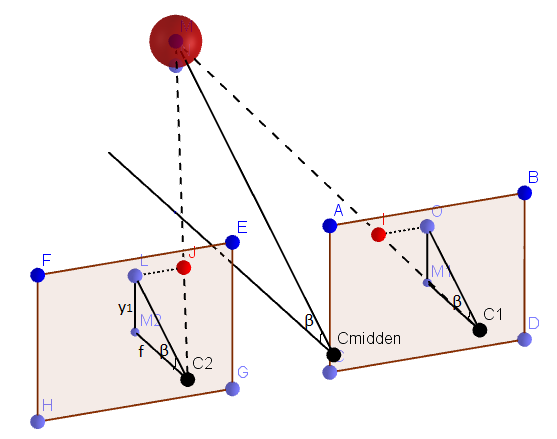
\includegraphics[width=1\textwidth]{RelatieveVerticaleHoek.png}
		\caption{Relatieve verticale hoek.}
		\label{fig:RelatieveVerticaleHoek}
	\end{minipage}%
	\caption*{In Figuur \ref{fig:RelatieveHorizontaleHoek} wordt de relatieve horizontale hoek tussen drone en doel weergegeven door \(\tan(\alpha) = \frac{x-\frac{c}{2}}{Z}\), voor de volledige uitwerking zie formule \ref{eq:RelatieveVerticaleHoekBegin} tot \ref{eq:RelatieveVerticaleHoekEind}.\\
		In Figuur \ref{fig:RelatieveVerticaleHoek} wordt de relatieve verticale hoek weergegeven tussen drone en doel. De relatie wordt gegeven door volgende formule: \(\tan(\beta) = \frac{y_1}{f}\).}
\end{figure}
\begin{figure}[h]
	\centering
	\begin{minipage}{.45\textwidth}
	\begin{center}
			Berekening brandpuntsafstand f:
	\end{center}
		\begin{equation} \label{eq:RelatieveVerticaleHoekBegin}
		\tan(\delta) = \frac{b}{f}
		\end{equation}
		\begin{equation} 
		f = \frac{b}{\tan(\delta)}
		\end{equation}
	\end{minipage}
	\begin{minipage}{.45\textwidth}
		\begin{center}
			Berekening afstand x:
		\end{center}
		\begin{equation} 
		\frac{x_2}{f} = \frac{x}{Z}
		\end{equation}
		\begin{equation} \label{eq:RelatieveVerticaleHoekEind}
		x = Z \cdot \frac{x_2}{f}	
		\end{equation}
	\end{minipage}%
\end{figure}
\\
Nadat de drone zijn positie bepaald heeft, kan hij zijn fouten (horizontale en verticale hoek en eventuele roll) bijsturen a.d.h.v. PI-controllers die beslissen over respectievelijk yaw, thrust en roll bewegingen. Meer info over de werking van de controllers wordt gegeven in sectie \ref{subsec: PI Controllers}. 
\\
\\
Nu rest enkel nog het bepalen van de pitch zodat er onder een ingestelde thrust voorwaarts richting de bol kan bewogen worden. Het eerste idee was om dit op basis van een snelheidscontroller te doen, aangezien de snelheid afhankelijk is van de pitch en hierdoor het controleerbaar zou zijn. De snelheid is echter niet te bepalen door de onbekende windkrachten en door de numeriek wiskundige beperkingen op het berekenen van afgeleiden. Hierdoor zou immers de fout te groot worden. Bijgevolg werd er overgegaan op een alternatief plan. Dit houdt in dat de drone pitcht met een rate op basis van een afstandscontroller. Deze legt altijd een doelafstand vast op een kleine afstand voor de drone zodat hij beperkt wordt tot telkens kleine afstanden overbruggen. Door de combinatie van de kleine afstanden en het feit dat de drone telkens terug horizontaal moet komen per overbrugde afstand, kan de snelheid laag gehouden worden. Wanneer er tegenwind is en de drone verder zou afwijken van zijn doelafstand, zal de afstandscontroller de drone toelaten om verder te pitchen om zo toch tegen de windkracht in zijn doel te bereiken.
\\
\\
Ten slotte moet dit proces herhaaldelijk worden uitgevoerd ten gevolge van de invloed van wind. De wind kan de drone namelijk uit koers brengen. Hierdoor zal de drone telkens zijn positie moeten herberekenen, zich opnieuw ori\"enteren en de controllers laten bijsturen.